\documentclass{thureport}
% =============================================
% Part 1 Edit the info
% =============================================

\newcommand{\major}{软件71}
\newcommand{\name}{骆炳君}
\newcommand{\stuid}{2017013573}
\newcommand{\newdate}{2019-4-15}
\newcommand{\newtitle}{用单色仪测定介质吸收曲线}
\newcommand{\dL}{\delta L}
\def\celsius{{\ensuremath{^\circ\hspace{-0.09em}\mathrm{C}}}}

% =============================================
% Part 1 Main document
% =============================================
\begin{document}
\thispagestyle{empty}
\begin{figure}[h]
	\begin{minipage}{0.65\linewidth}
		\centerline{
\includegraphics[width=\linewidth]{head.jpg}}
	\end{minipage}
	\hfill
	\begin{minipage}{.3\linewidth}
		\raggedleft
		\begin{tabular*}{.8\linewidth}{ll}
			班级: & \underline\major   \\
			姓名: & \underline\name    \\
			学号: & \underline\stuid   \\
			日期: & \underline\newdate
		\end{tabular*}
	\end{minipage}
\end{figure}
 
\begin{table}[!htbp]
	\centering\large
	实验名称: \underline\newtitle
\end{table}

\tableofcontents
% =============================================
% Part 2 Main document
% =============================================
\newpage

\section{实验目的}
\begin{clause}
	\item 学习掌握光栅单色仪的基本构造和使用方法.
	\item 学习了解介质光谱特性,掌握测量介质的吸收/透射曲线的原理和方法.
	\item 学习使用计算机作图法处理实验数据.
\end{clause}

\section{实验原理}
\subsection{介质的透射率和吸收系数}
一束波长为$\lambda$、入射光强为$I_0$的单色平行光垂直入射到厚度为$d$的介质板上,设从界面1反射光的光强为$I_R$,从界面1向介质内透射光的光强为$I_1$,入射到界面2的光强为$I_2$,界面2的透射光的光强为$I_T$.

定义介质板的光谱外透射率$T$和光谱透射率$T_i$为

$$T=\frac{I_T}{I_0},\ T_i=\frac{I_2}{I_1}$$

假定介质内部无散射,光谱透射率$T_i$与介质厚度$d$满足

$$T_i=e^{-\alpha d}$$

其中$\alpha$被称为介质的线性吸收系数,其值不仅与介质有关,而且与入射光的波长$\lambda$有关,$\alpha$与$\lambda$的关系曲线被称为吸收曲线.

\subsection{测量光谱透射率和吸收系数}
设光在单一界面上的反射率为$R$,则透射光的光强为
$$
\begin{aligned}
I_T&=\sum_{i=1}^\infty I_{Ti}\\
&=\sum_{i=1}^\infty I_0(1-R)^2R^{2(i-1)}e^{-(2i-1)\alpha d}\\
&=\frac{I_0(1-R)^2e^{-\alpha d}}{1-R^2e^{-2\alpha d}}
\end{aligned}
$$

通过测量同一材料($\alpha$相同),表面性质相同($R$相同),但厚度不同的两块试样的光谱外透射率可以计算得出介质的$T_i$和$\alpha$.

设两块试样的厚度分别为$d_1$和$d_2$($d_2>d_1$),光谱外透射率分别为$T_1$和$T_2$,由上式可得

$$\frac{T_2}{T_1}=\frac{e^{-\alpha d_2}(1-R^2e^{-2\alpha d_1})}{e^{-\alpha d_1}(1-R^2e^{-2\alpha d_2})}\approx e^{-\alpha(d_2-d_1)}$$

在本实验中使用光电池和微电流放大器测量光强,设$T_1$和$T_2$对应的微电流放大器显示值为$n_1$和$n_2$,可得

$$T_i=\frac{n_2}{n_1}$$

$$\alpha=\frac{\ln{T_1}-\ln{T_2}}{d_2-d_1}=\frac{\ln{n_1}-\ln{n_2}}{d_2-d_1}$$

\section{实验仪器}
\begin{clause}
	\item WDG30型光栅单色仪
	\item 汞灯GP20Hg
	\item 溴钨灯及其电源
	\item 会聚透镜L
	\item 不同厚度的钕玻璃样品
\end{clause}

\section{实验步骤}
\subsection{校对单色仪的波长示值准确度}
\begin{clause}
	\item 调节单色仪手轮,使波长读数在577.0到579.1mm之间.
	\item 将汞灯放在入射狭缝前,把$S_1$、$S_2$宽度调至约2mm,观察黄色谱线.
	\item 关小入射狭缝$S_1$,使两条谱线分开且尽量细、亮.
	\item 关小出射狭缝$S_2$,同时微动手轮,使狭缝宽度与谱线同宽.
	\item 微动手轮使谱线位于视野中央,读出此时手轮示数.
	\item 转动手轮到其他谱线,测全汞灯4条谱线的对应示值,与标准值进行比较.
\end{clause}

\subsection{调节狭缝宽度}
\begin{clause}
	\item 调节单色仪手轮,使波长读数在577.0到579.1mm之间.
	\item 用显微镜迎着出射光方向观察$S_2$上的两条黄色谱线,微动手轮使谱线移到视野中央.
	\item 调节入射狭缝$S_1$宽度,使两条谱线刚好分开.
	\item 调节出射狭缝$S_2$宽度,同时微调手轮,使其中一条谱线在缝中央且与缝同宽.
\end{clause}

\subsection{调节溴钨灯光路}
\begin{clause}
	\item 调节会聚透镜和溴钨灯的位置,使透镜距狭缝约18cm,溴钨灯距透镜约9cm.
	\item 打开溴钨灯电源,把手轮调到610.0mm,进行共轴调节,使透镜像位于狭缝中间且全部变亮.
	\item 装上样品和光电池探测器,打开微电流放大器,调节溴钨灯电流使微电流放大器示值大于1.900.
\end{clause}

\subsection{测量钕玻璃的吸收曲线}
\begin{clause}
	\item 定性观察钕玻璃对各色光的吸收情况,从610.0nm到550.0nm转动手轮大致测定吸收峰位置.
	\item 转动手轮,从610.0nm到508.0nm每隔2nm记录一次放大器示值,在吸收峰附近每0.5nm测量一次.
	\item 更换为厚样品,重复(2)中测量过程,其测量点波长应与(2)中相同.
\end{clause}

\subsection{实验注意事项}
\begin{clause}
	\item 溴钨灯电流不超过2.50A.
	\item 转动手轮波长不应超出400.0到800.0nm范围.
	\item 两狭缝$S_1$和$S_2$的宽度目测既不能超过2mm,也不能完全闭合,否则会损坏狭缝机构.
\end{clause}

\section{数据处理}
\subsection{波长示值的校对}
% Table generated by Excel2LaTeX from sheet 'Sheet1'
\begin{table}[htbp]
    \centering
      \begin{tabular}{|c|c|c|c|c|}
      \hline
      标准值(nm)   & 579.1  & 577.0  & 546.1  & 435.8  \bigstrut\\
      \hline
      测量值(nm)   & 578.0  & 575.9  & 545.1  & 434.8  \bigstrut\\
      \hline
      偏差$\Delta\lambda$(nm)    & 1.1   & 1.1   & 1.0   & 1.0  \bigstrut\\
      \hline
      \end{tabular}%
  \end{table}%  

$\Delta\lambda$间的差值小于$0.2nm$,符合要求.

$$\overline{\Delta\lambda}=\frac{1.1+1.1+1.0+1.0}{4}=1.05(nm)$$

\subsection{测定钕玻璃的吸收特性}
将实验所得数据进行整理,得到下表:

其中$\lambda=\lambda_0+\overline{\Delta\lambda}$, $\alpha=\frac{\ln{n_1}-\ln{n_2}}{d_2-d_1}$, $d_2=1mm$, $d_1=0.5mm$.

\begin{table}[H]
    \centering
      \begin{tabular}{|c|c|c|c|c|c|c|c|c|c|}
      \hline
      $\lambda_0(nm)$ & $\lambda(nm)$ & $n_1$   & $n_2$   & $\alpha(mm^{-1})$ & $\lambda_0(nm)$ & $\lambda(nm)$ & $n_1$   & $n_2$   & $\alpha(mm^{-1})$ \bigstrut\\
      \hline
    610.0  & 611.05  & 1.970  & 1.727  & 0.26330  & 572.5  & 573.55  & 0.661  & 0.232  & 2.09403  \bigstrut\\
    \hline
    608.0  & 609.05  & 1.908  & 1.642  & 0.30028  & 572.0  & 573.05  & 0.665  & 0.238  & 2.05503  \bigstrut\\
    \hline
    606.0  & 607.05  & 1.854  & 1.557  & 0.34917  & 571.5  & 572.55  & 0.681  & 0.252  & 1.98827  \bigstrut\\
    \hline
    604.0  & 605.05  & 1.778  & 1.440  & 0.42169  & 571.0  & 572.05  & 0.716  & 0.285  & 1.84238  \bigstrut\\
    \hline
    602.0  & 603.05  & 1.683  & 1.300  & 0.51643  & 570.5  & 571.55  & 0.755  & 0.329  & 1.66132  \bigstrut\\
    \hline
    600.0  & 601.05  & 1.575  & 1.145  & 0.63770  & 570.0  & 571.05  & 0.819  & 0.398  & 1.44326  \bigstrut\\
    \hline
    598.0  & 599.05  & 1.464  & 0.982  & 0.79867  & 568.0  & 569.05  & 1.147  & 0.796  & 0.73061  \bigstrut\\
    \hline
    596.0  & 597.05  & 1.323  & 0.807  & 0.98867  & 566.0  & 567.05  & 1.358  & 1.135  & 0.35876  \bigstrut\\
    \hline
      \end{tabular}%
\end{table}%

\begin{table}[H]
    \centering
      \begin{tabular}{|c|c|c|c|c|c|c|c|c|c|}
      \hline
      $\lambda_0(nm)$ & $\lambda(nm)$ & $n_1$   & $n_2$   & $\alpha(mm^{-1})$ & $\lambda_0(nm)$ & $\lambda(nm)$ & $n_1$   & $n_2$   & $\alpha(mm^{-1})$ \bigstrut\\
      \hline
      594.0  & 595.05  & 1.125  & 0.584  & 1.31127  & 564.0  & 565.05  & 1.429  & 1.269  & 0.23749  \bigstrut\\
    \hline
    592.0  & 593.05  & 0.947  & 0.415  & 1.65004  & 562.0  & 563.05  & 1.433  & 1.299  & 0.19635  \bigstrut\\
    \hline
    590.0  & 591.05  & 0.828  & 0.318  & 1.91392  & 560.0  & 561.05  & 1.421  & 1.300  & 0.17799  \bigstrut\\
    \hline
    588.5  & 589.55  & 0.750  & 0.258  & 2.13423  & 558.0  & 559.05  & 1.400  & 1.291  & 0.16211  \bigstrut\\
    \hline
    588.0  & 589.05  & 0.712  & 0.231  & 2.25132  & 556.0  & 557.05  & 1.378  & 1.276  & 0.15381  \bigstrut\\
    \hline
    587.5  & 588.55  & 0.675  & 0.205  & 2.38341  & 554.0  & 555.05  & 1.352  & 1.253  & 0.15209  \bigstrut\\
    \hline
    587.0  & 588.05  & 0.636  & 0.183  & 2.49142  & 552.0  & 553.05  & 1.326  & 1.231  & 0.14868  \bigstrut\\
    \hline
    586.5  & 587.55  & 0.601  & 0.166  & 2.57321  & 550.0  & 551.05  & 1.302  & 1.211  & 0.14491  \bigstrut\\
    \hline
    586.0  & 587.05  & 0.567  & 0.148  & 2.68629  & 548.0  & 549.05  & 1.278  & 1.184  & 0.15280  \bigstrut\\
    \hline
    585.5  & 586.55  & 0.545  & 0.136  & 2.77626  & 546.0  & 547.05  & 1.248  & 1.155  & 0.15488  \bigstrut\\
    \hline
    585.0  & 586.05  & 0.524  & 0.124  & 2.88242  & 544.0  & 545.05  & 1.215  & 1.118  & 0.16641  \bigstrut\\
    \hline
    584.5  & 585.55  & 0.516  & 0.122  & 2.88417  & 542.0  & 543.05  & 1.181  & 1.068  & 0.20115  \bigstrut\\
    \hline
    584.0  & 585.05  & 0.522  & 0.125  & 2.85871  & 540.0  & 541.05  & 1.136  & 1.015  & 0.22525  \bigstrut\\
    \hline
    583.5  & 584.55  & 0.537  & 0.135  & 2.76145  & 538.0  & 539.05  & 1.082  & 0.934  & 0.29418  \bigstrut\\
    \hline
    583.0  & 584.05  & 0.566  & 0.154  & 2.60328  & 536.0  & 537.05  & 1.019  & 0.836  & 0.39590  \bigstrut\\
    \hline
    582.5  & 583.55  & 0.597  & 0.173  & 2.47725  & 534.0  & 535.05  & 0.935  & 0.724  & 0.51151  \bigstrut\\
    \hline
    582.0  & 583.05  & 0.634  & 0.196  & 2.34787  & 532.0  & 533.05  & 0.861  & 0.624  & 0.64389  \bigstrut\\
    \hline
    581.5  & 582.55  & 0.666  & 0.219  & 2.22444  & 530.0  & 531.05  & 0.815  & 0.564  & 0.73627  \bigstrut\\
    \hline
    581.0  & 582.05  & 0.716  & 0.250  & 2.10444  & 528.0  & 529.05  & 0.782  & 0.532  & 0.77042  \bigstrut\\
    \hline
    580.5  & 581.55  & 0.743  & 0.269  & 2.03197  & 526.0  & 527.05  & 0.776  & 0.533  & 0.75126  \bigstrut\\
    \hline
    580.0  & 581.05  & 0.773  & 0.294  & 1.93340  & 524.0  & 525.05  & 0.776  & 0.550  & 0.68847  \bigstrut\\
    \hline
    578.0  & 579.05  & 0.776  & 0.301  & 1.89408  & 522.0  & 523.05  & 0.802  & 0.615  & 0.53097  \bigstrut\\
    \hline
    576.5  & 577.55  & 0.734  & 0.272  & 1.98541  & 520.0  & 521.05  & 0.824  & 0.663  & 0.43479  \bigstrut\\
    \hline
    576.0  & 577.05  & 0.719  & 0.261  & 2.02668  & 518.0  & 519.05  & 0.807  & 0.656  & 0.41433  \bigstrut\\
    \hline
    575.5  & 576.55  & 0.711  & 0.255  & 2.05082  & 516.0  & 517.05  & 0.777  & 0.618  & 0.45790  \bigstrut\\
    \hline
    575.0  & 576.05  & 0.695  & 0.250  & 2.04490  & 514.0  & 515.05  & 0.736  & 0.566  & 0.52527  \bigstrut\\
    \hline
    574.5  & 575.55  & 0.686  & 0.245  & 2.05924  & 512.0  & 513.05  & 0.715  & 0.549  & 0.52837  \bigstrut\\
    \hline
    574.0  & 575.05  & 0.678  & 0.241  & 2.06870  & 510.0  & 511.05  & 0.716  & 0.568  & 0.46312  \bigstrut\\
    \hline
    573.5  & 574.55  & 0.672  & 0.235  & 2.10135  & 508.0  & 509.05  & 0.724  & 0.600  & 0.37572  \bigstrut\\
    \hline
    573.0  & 574.05  & 0.662  & 0.231  & 2.10570  &       &       &       &       &  \bigstrut\\
    \hline
      \end{tabular}%
\end{table}%
  
利用以上数据可作出钕玻璃的吸收曲线(见附录),根据实验数据和吸收曲线可以明显地发现钕玻璃的两个吸收峰,分别是
$$\lambda_1=585.55nm,\ \alpha_1=2.88417$$
$$\lambda_1=574.05nm,\ \alpha_1=2.10570$$

\section{实验小结}
本次实验使用了光栅单色仪等精密光学仪器,校正仪器偏差和调节仪器参数也是实验操作中最具挑战性的部分.在实验过程中暴露了我的很多不足之处,例如对实验原理不够理解,对实验仪器不够熟悉等.感谢助教的悉心指导!

\section{思考题}
\subsection*{1.}
汞灯在可见光波段有4条谱线,且其波长已经被较为精确地测定,适合用来校对单色仪的波长示值.

溴钨灯能够产生连续谱,而且光效高,寿命长,具有很高的输出稳定性,光谱覆盖范围宽,适合用来测量吸收曲线.

\subsection*{2.}
狭缝宽度越小,出射光的单色性越小,但过小的宽度会使得光强不够,导致观察困难.因此需要平衡单色性和光强的关系,一般应保持出射狭缝宽度和入射狭缝宽度相等,才能使出射光具有最好的单色性和最大的光强.

\subsection*{3.}
因为在该实验中采用了控制变量的方法,在使用不同厚度的钕玻璃片时控制光源、波长和光电池的状态保持相同,可以消除其他因素对微电流放大器显示值的影响,没有必要考虑后两者.

\subsection*{4.}
在光栅单色仪中,出射光的波长$\lambda$满足

$$\lambda=d(\sin\theta-\sin i)$$

当光栅的角度转过$\alpha$时,$\theta=\theta_0+\alpha$,$i=i_0-\alpha$,手轮移动的距离$x=k\sin\alpha$.

由此可得

$$\frac{\lambda}{x}=\frac{d(\sin(\theta_0+\alpha)-\sin(i_0-\alpha))}{k\sin\alpha}=\frac{d}{k}(\cos\theta_0+\cos i_0)$$

因为$\lambda$与$x$成线性关系,所以把光栅单色仪称为线性分光仪器.

\newpage
\section{吸收曲线}
\begin{figure}[H]
	\centering
	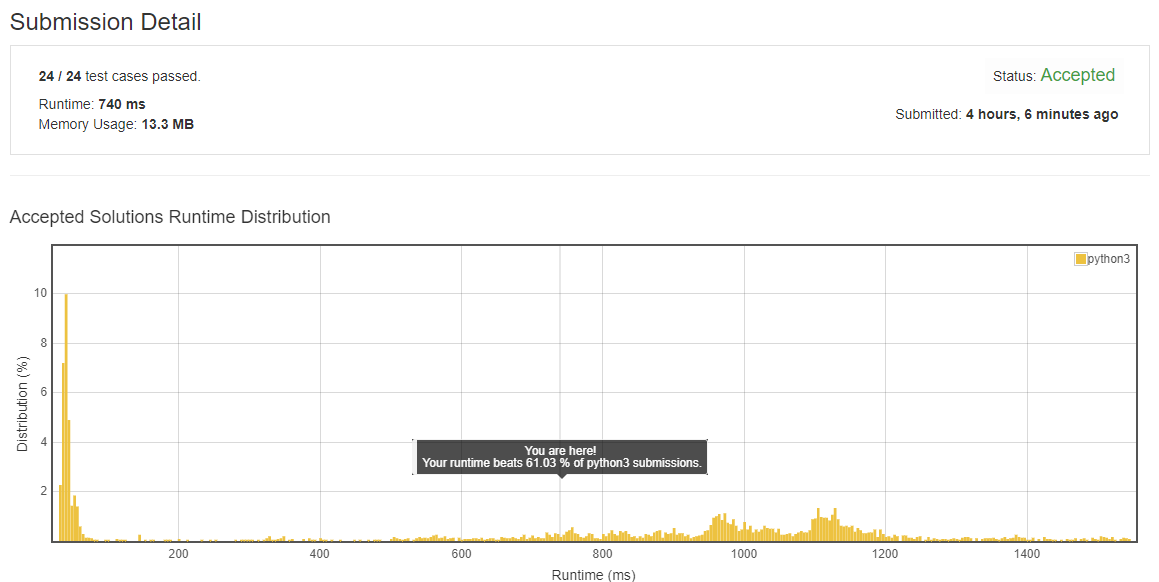
\includegraphics[width=0.8\linewidth]{figure1.png}
\end{figure}

\newpage
\section{原始数据表格}

\end{document}